\label{chap:background}

This chapter discusses relevant background information toward the goal of implementing a packetized display protocol (PDP) architecture for Infrared Scene Projector systems (IRSPs). First, it gives an overview of what constitutes an IRSP system. Following this, it provides a general discussion of how common display protocols work to send pixel data to a display system (e.g. a television). Finally, it discusses how these protocols are utilized within an IRLED project system including discussion of example scenarios.

%FIXME: Add new information above

\section{IRLED Projector Systems}
\label{sec:irled_projector_systems}
    \begin{figure}
        \centering
        %includegraphs[trim=L B R T]
        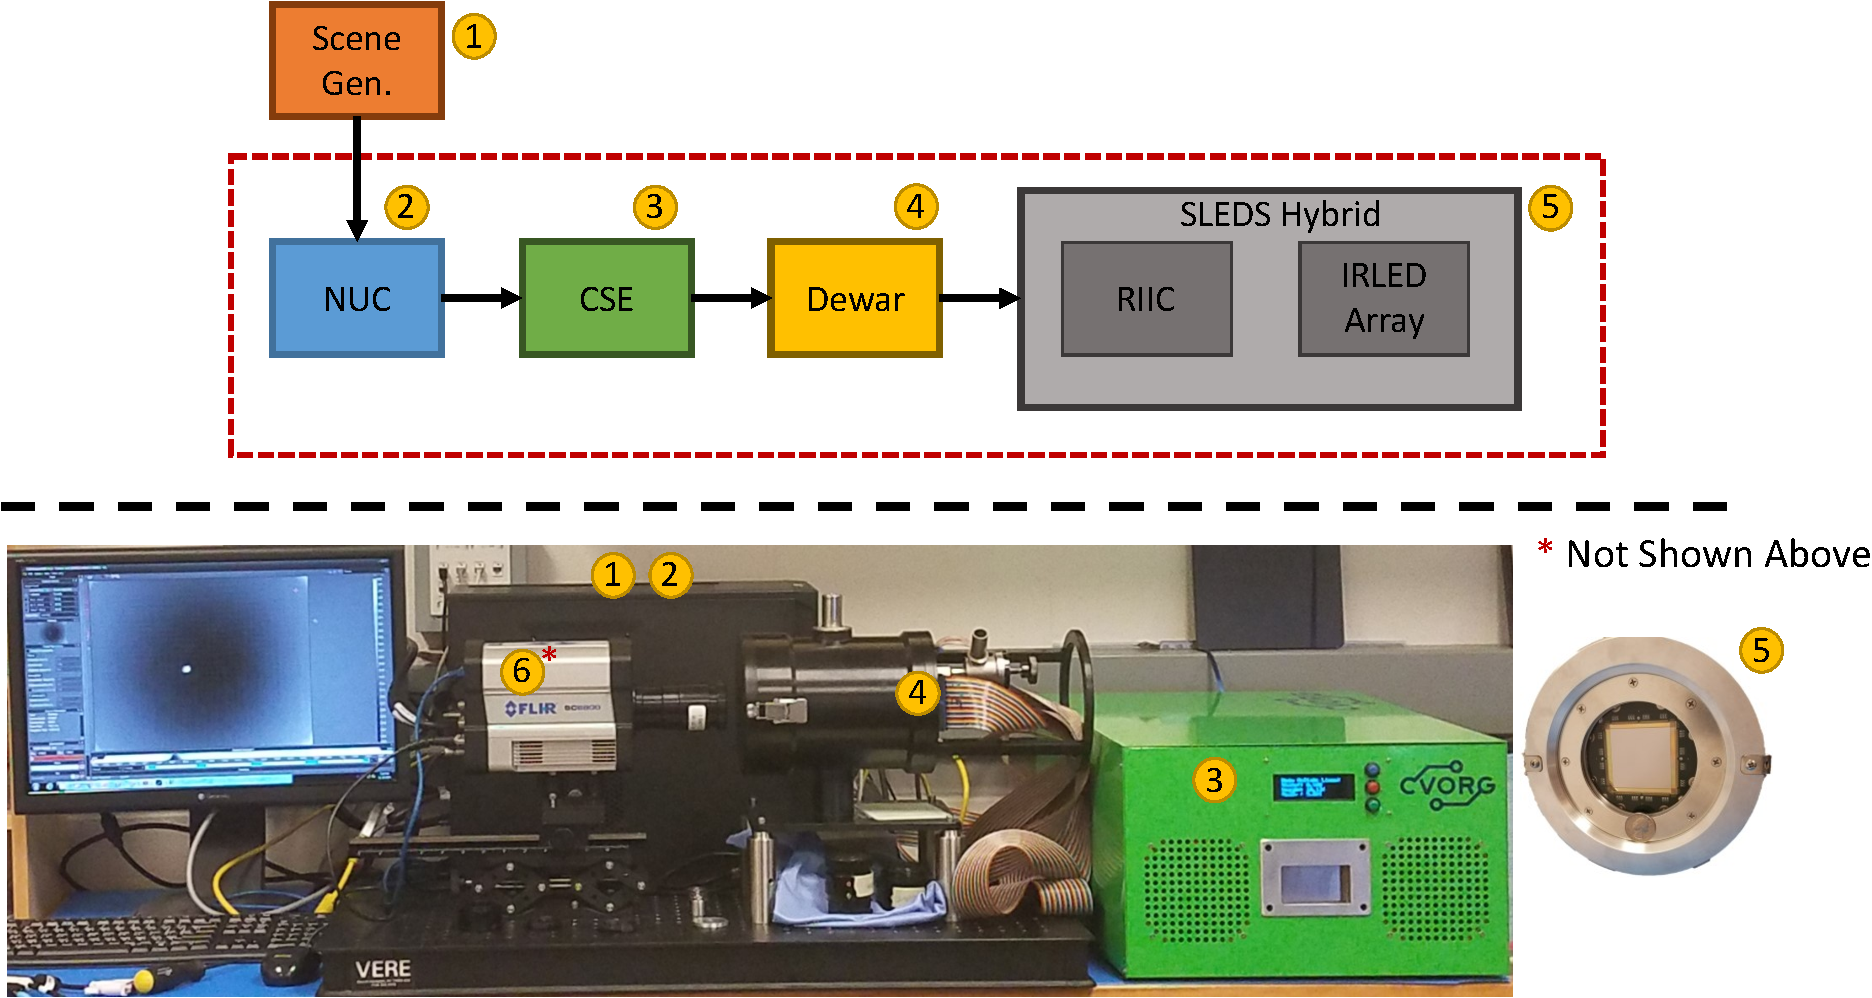
\includegraphics[trim=0.45in 1.25in 0.0in 0in,width=1.0\textwidth]{fig/sleds_system.pdf}
        \caption{IRLED Scene Projector System}
        \label{fig:sleds_system}
    \end{figure}

    IRLED based IRSPs are made up light emitting diodes (LEDs) that emit light in the IR spectrum\cite{biard1966semiconductor}. Since their inception they have been utilized in various fields such as medical sensing\cite{MonteiroEtAl2011,MEEKS1998433,Sadick2009,takhtfooladi2015effects,yamanishi1995respiration}; tracking; and localization\cite{PlotogVladescu2015,Kimon2001,SCHOLZ20151233,WalshDaemsSteckel2015,zeylikovich2003mid}, and communication\cite{CossuEtAl2014,escobosa2004ir,GeorgopoulosKormakopoulos1986,sohn2007localization,JangEtAl2012}.

    Modern IRLED projectors are an emerging technology with various applications within the IR sensor testing community. A complete IRLED based IRSP system consist of various technologies and processes as shown in Figure~\ref{fig:sleds_system}. One denotes the scene generation and two the non-uniformity correction (NUC) process. These are where pixel data representing IR scenes is fed to a system for display. The NUC process corrects for physical and thermal non-uniformity\cite{BarakhshanEtAl2017} in an IRLED array\cite{BarakhshanEtAl2018}. Three denotes the close support electronics\cite{ejzak4} which are responsible for converting a digital representation of a scene into analog signaling that goes directly to an array. Four indicates the dewar\cite{lang1, MarksEtAl2017} or vaccum chamber which houses an IRLED array and is utilized to keep it below ambient temperatures or at cryogenic temperature ranges. Five indicates an IRLED hybrid which consist of a Read-in Integrated Circuit (RIIC)\cite{HernandezEtAl2017} used to address an IRLED array and the array itself. Analog signals coming from the CSE go into the dewar, and then are mapped using the RIIC, which results in specific IRLEDs within an array being driven. Six indicates an IR recording apparatus of some sort utilized to record IR data from an array. Synchronization between source generation, display, and recording is maintained via explicit synchronization signaling. Often Camera Link serial communication\cite{CameraLink2000, zhu2008design} is used to capture imagery. My lab setup uses FLIR Systems High-speed IR Cameras\cite{FLIR1, FLIR2}. The red dotted lines show what is provided within an IRLED system; where as, scene generation is usually application specific and thus excluded. In the image, Scene Generation and NUC are performed within the same machine.

    Figure~\ref{fig:sleds_timeline} shows the development timeline for IRLED Projector technology. In 2008, the world's first IRLED array called the Superlattice Light Emitting Diodes (SLEDs) array was completed\cite{ahmed1}. This device was a hybridized combination of a 68 by 68 IRLED wafer bonded to a RIIC wafer\cite{das2} providing the electronics to drive the array. Initial testing was done by hand prior the design and implementation of the overall drive system which was completed in 2011. Following this, an increased IRLED wafer of 512x512 size was fabricated in 2014\cite{norton1}. The combination of the array with the drive system resulted in SLEDS (Superlattice Light Emitting Diode System), the first functioning IRLED projector system in the world. Further efforts culminated in two IRLED projector systems in 2016. The first, TCSA (Two Color SLEDS Array), a 512 by 512 sized array\cite{McGeeEtAl2015, ejzak1, ejzak2, EjzakEtAl2016, RickerEtAl2017} included support for driving the LEDs at two separate wavelength bands (denoted as 2-colors in Figure~\ref{fig:sleds_timeline}. The second, NSLEDS (N\footnote{The N originally stood for Nightglow, before the device was retargeted to Midwave-IR.} Superlattice Infrared Light Emitting Diode System), a 1024 by 1024 sized array\cite{benedict1} doubled the total number of pixels supported. Additionally, these systems demonstrated the beginnings of a modular IR Scene Projection (IRSP) platform\cite{BrowningEtAl2019}. A further increase in size and efficiency occurred in 2018 with the world's first 2048 by 2048 pixel array, HDILED (High Definition Infrared LED). A visual representation of the pixel ratios is shown in Figure~\ref{fig:tcsa_nsleds_hdiled_array_ratio}

    TCSA represented a novel step forward in terms of IRLED array technology. It incorporated a multiple color pixel design within a 1.3in\textsuperscript{2} package consisting of two overlayed LEDs per pixel to enable emission in multiple wave-length spectrums, as well as, an increase in the number of analog channels from 4 to 16 to allow for more pixels to be driven at a time. It targeted a speed of \mbox{1 KHz} operation. NSLEDS used the same size wafer as a TCSA, but decreased the pixel pitch from 48 to 24 microns and incorporated a single color pixel design instead of the multiple color design of the original, these changes allowed for the pixel resolution to be doubled paving the way toward larger format IRLED IRSPs. Additionally, NSLEDS targeted \mbox{500 Hz} operation. HDILED increased the package size to 2.3in\textsuperscript{2} and doubled the resolution while utilizing a similar RIIC architecture to the prior two arrays. It targeted \mbox{250 Hz} operation. The interleaved write process of each array will be discussed in detail in Section~\ref{sec:array_Interleaved_write_process}.

    \begin{figure}
        \centering
        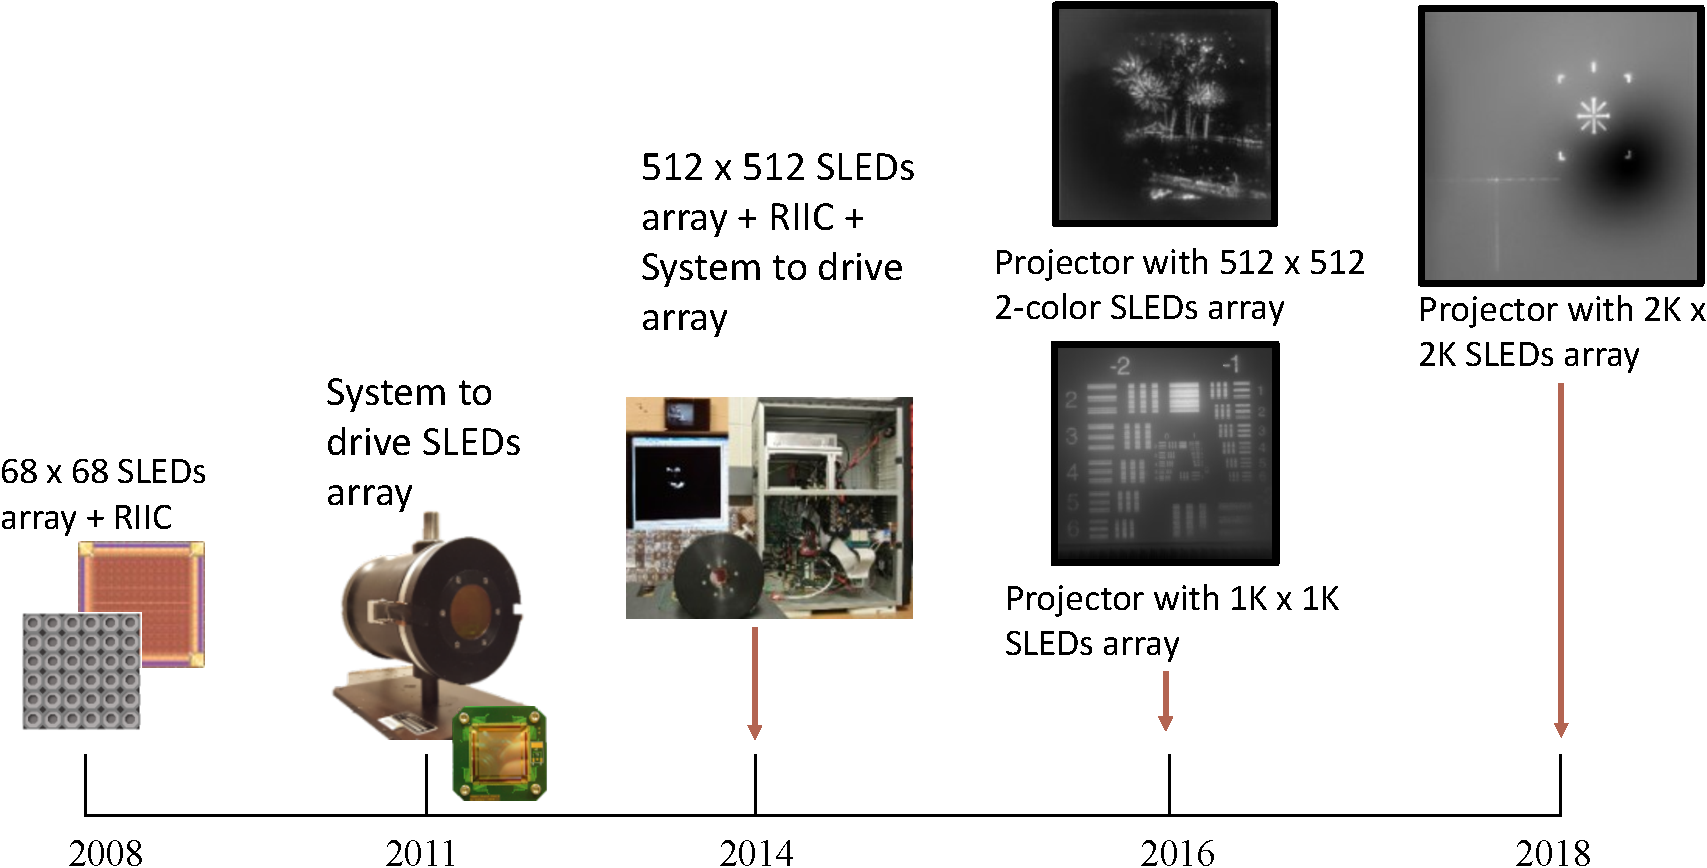
\includegraphics[trim=0.5in 0.5in 0.5in 1.5in,width=1.0\textwidth]{fig/sleds_timeline.pdf}
        \caption{IRLED Projector Technology Development Timeline Overview}
        \label{fig:sleds_timeline}
    \end{figure}

    \begin{figure}
        \centering
        %includegraphs[trim=L B R T]
        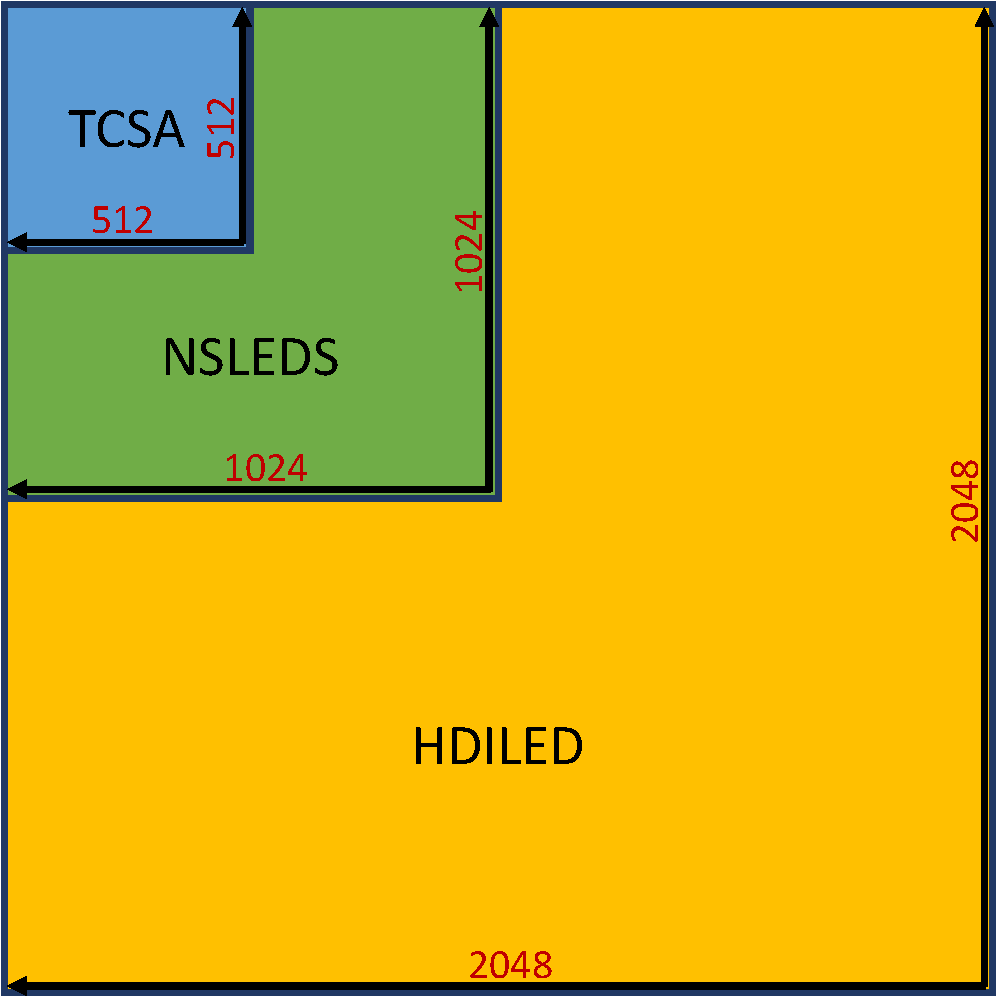
\includegraphics[trim=0.5in 0.5in 0.5in 1.5in,width=1.0\textwidth]{fig/tcsa_nsleds_hdiled_array_ratio.pdf}
        \caption{SLEDs Array Pixel Ratios}
        \label{fig:tcsa_nsleds_hdiled_array_ratio}
    \end{figure}


    Figure~\ref{fig:typical_projection} shows a typical projection process utilized within an IRLED IRSP. Each step operates at a static rate. A scene projector will perform scene generation utilizing a GPU typically. Following this, imagery will undergo non-uniformity correction by utilizing a NUC table created by analyzing the non-uniformity on a given array. After which, a digital to analog conversion will occur for each value displayed on a projector.

    \begin{figure}
        \centering
        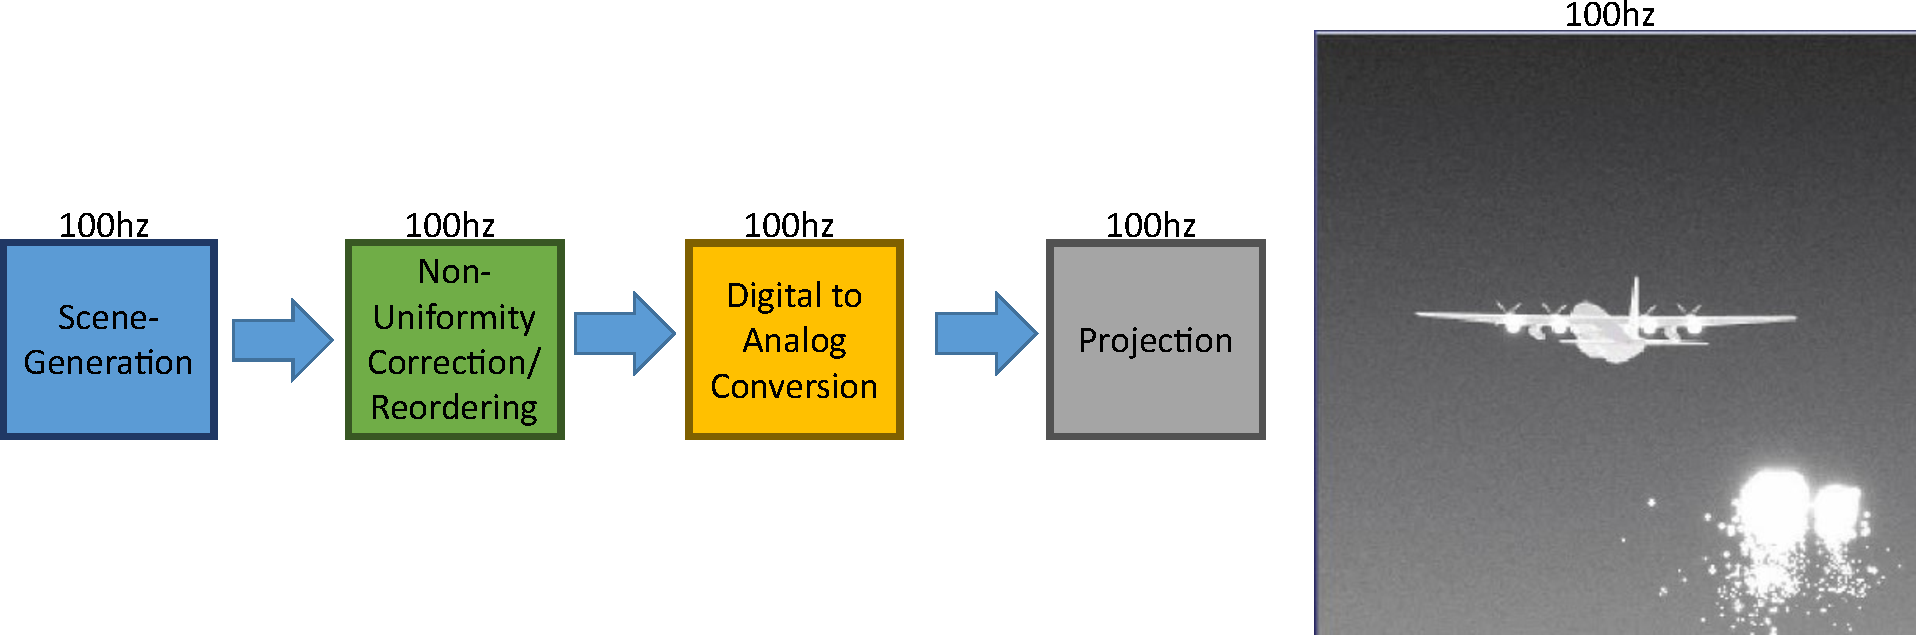
\includegraphics[trim=0in 0.5in 0in 1.5in,width=1.0\textwidth]{fig/typical_projection_system.pdf}
        \caption{Typical IRLED Projection Process}
        \label{fig:typical_projection}
    \end{figure}

    The NUC process compensates for any physical defects that may cause non-linear variation in light emission from different diodes on a given array, thus, allowing for uniform emission across a given spectrum. There are number of different ways this linearization may be performed\cite{BrowningEtAl2016, LandwehrEtAl2017, BarakhshanEtAl2019}, the details of which are beyond the scope of this work. After non-uniformity correction, imagery is converted pixel by pixel from digital to analog to drive the physical pixels at a given intensity on the array. The design of the digital to analogy chain of an IRLED IRSP is another important challenge as the analog bandwidth\footnote{The rise and fall time of digital in to analog out conversion.} plays an important role in determining the maximum speed a system can operate at, as well as, the bit resolution of an array. Additionally, timing variance and potential differences in performance between analog channels need to be analyzed and minimized through design and tuning. In SLEDs system, the analog chain is contained within the CSE. While outside of the scope of this work, it is worth noting that, a poorly behaving analog chain can introduce undesirable non-linear distortion in analog signaling resulting in non-linear projection \cite{freeman1977slewing, gordon1978linear, ChanEtAl2008}.

    Similarly, the internal analog timings of an array's RIIC plays a critical role in this as well. One that may be considered even more crucial given that once an array is fabricated and bonded, it cannot be later modified. In contrast, a faster and more precise analog chain could be implemented at a later point in time for an existing array.


\section{Close Support Electronics}
    \label{sec:close_support_electronics}
    As mentioned briefly in Section~\ref{sec:irled_projector_systems}, a CSE is needed to drive IRLED arrays. Conceptually, A CSE is an interface that converts digital display data to an array specific format in order to produce IR imagery. It further provides power for an array, and regulates the current in order to safe guard arrays from physical damage due to misconfiguration or heating.

    The TCSA, NSLEDS, and HDILED arrays can all be driven using the same electronics. Figure~\ref{fig:sleds_block} shows the internal components of the CSE broken out in green. A display system drives a CSE using two HDMI inputs in parallel to provide more physical bandwidth. Typically, these will each carry half of a frame segmented either vertically or horizontally. Two inputs are utilized to increase the system bandwidth and achieve higher frame-rates. Each hdmi input decodes the video signals in parallel and the output pixels are buffered into the main FPGA board which houses a Xilinx Vertex 6 FPGA\cite{XILINX1}.

    \begin{figure}
        \centering
        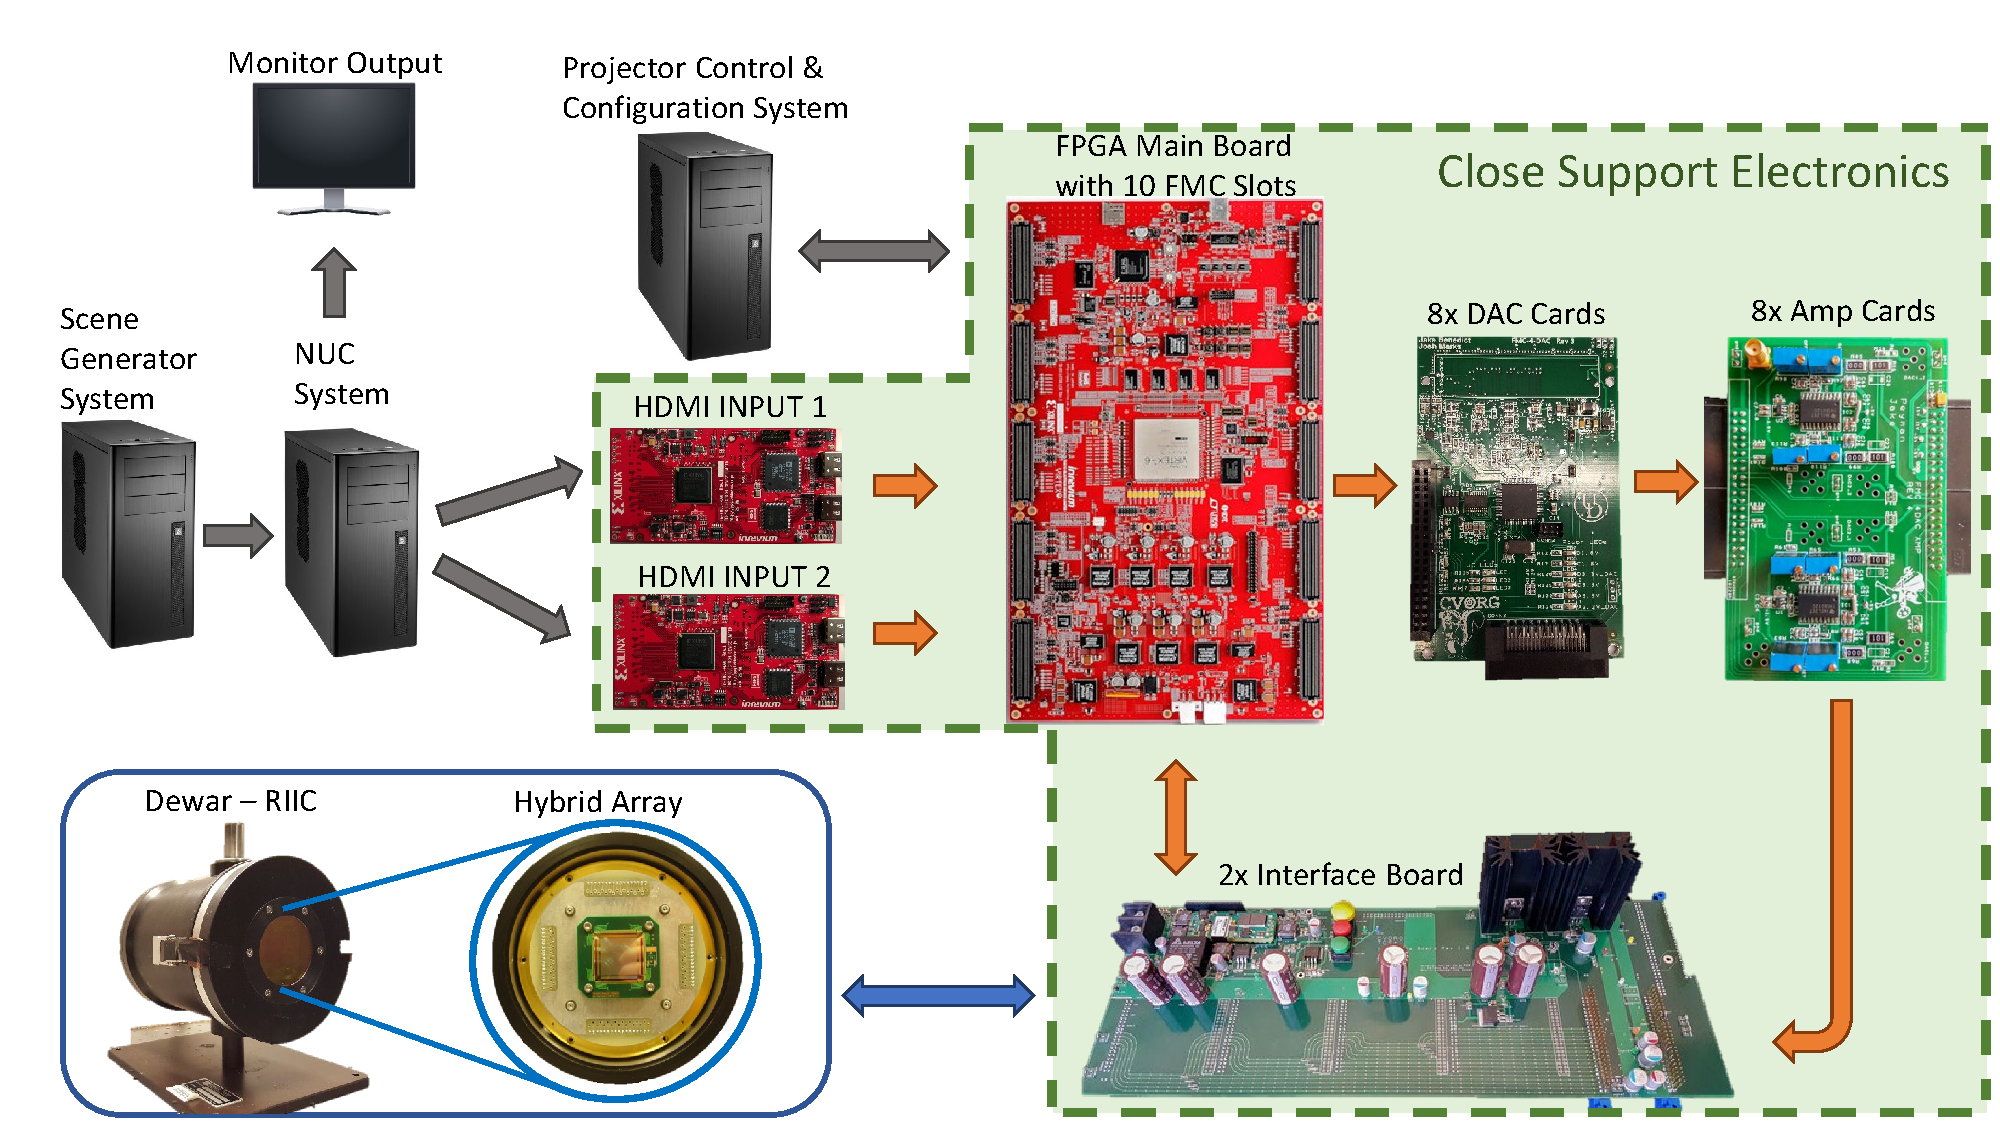
\includegraphics[width=1.0\textwidth]{fig/sleds_block.pdf}
        \caption{SLEDS System Block Diagram}
        \label{fig:sleds_block}
    \end{figure}

    Once enough data is buffered, the firmware will then control the write process to drive the 8 DAC cards which each house 2 16-bit DAC integrated circuits per card, with each circuit consisting of 2 channels per DAC. The output signals are then amplified and routed to the array through ribbon cables. Figure~\ref{fig:nessie_enclosure_internals} shows the components installed within a CSE.

    Multiple CSEs can be utilized to drive specific sections of an array as will be discussed briefly during

    Additional control signals provided by the firmware and routed to the RIIC are discussed in Section~\ref{sec:array_Interleaved_write_process}. The specifics of the PDP firmware architectures write process are discussed in Chapter~\ref{chap:implementation}.

    \begin{figure}
        \centering
        \includegraphics[width=0.7\textwidth]{fig/nessie_enclosure_internals.jpg}
        \caption{CSE Internals}
        \label{fig:nessie_enclosure_internals}
    \end{figure}

\section{Array Interleaved Write Process}
    \label{sec:array_Interleaved_write_process}
    As will be discussed in Section~\ref{sec:classical_display_protocols}, while all current IRSP arrays utilize some display protocol technology that is decoded in order to drive an array's pixels, arrays may utilize different internal drawing mechanisms for driving the pixels. This section discusses the details of those mechanisms within the TCSA, NSLEDS, and HDILED arrays for conceptual purposes, and while the details may differ for other arrays, the overall raster write process is generalizable.

    %FIXME: add proper citation for Tianne paper when published
    The TCSA, NSLEDS, and HDILED arrays are organized into four quadrants as shown in Figure~\ref{fig:tcsa_nsleds_hdiled_quads}. Each quadrant is organized into a given number of pixels with TCSA housing 256 by 256, NSLEDS housing 512 by 512, and HDILED housing 1024 by 1024 per quadrant. There are number of input signals necessary to drive an array. These are {\em a 4 bit quadrant write enable}, {\em X address}, {\em Y address}, {\em LOAD bit}, {\em 16 Strong/Weak drive strength bit}, {\em array reset bit}, and {\em analog signaling lines which charges the pixels being addressed}. The quadrant write enable, X address, Y address, and LOAD signals are all utilized for addressing the array.

    \begin{figure}
        \centering
        %includegraphs[trim=L B R T]
        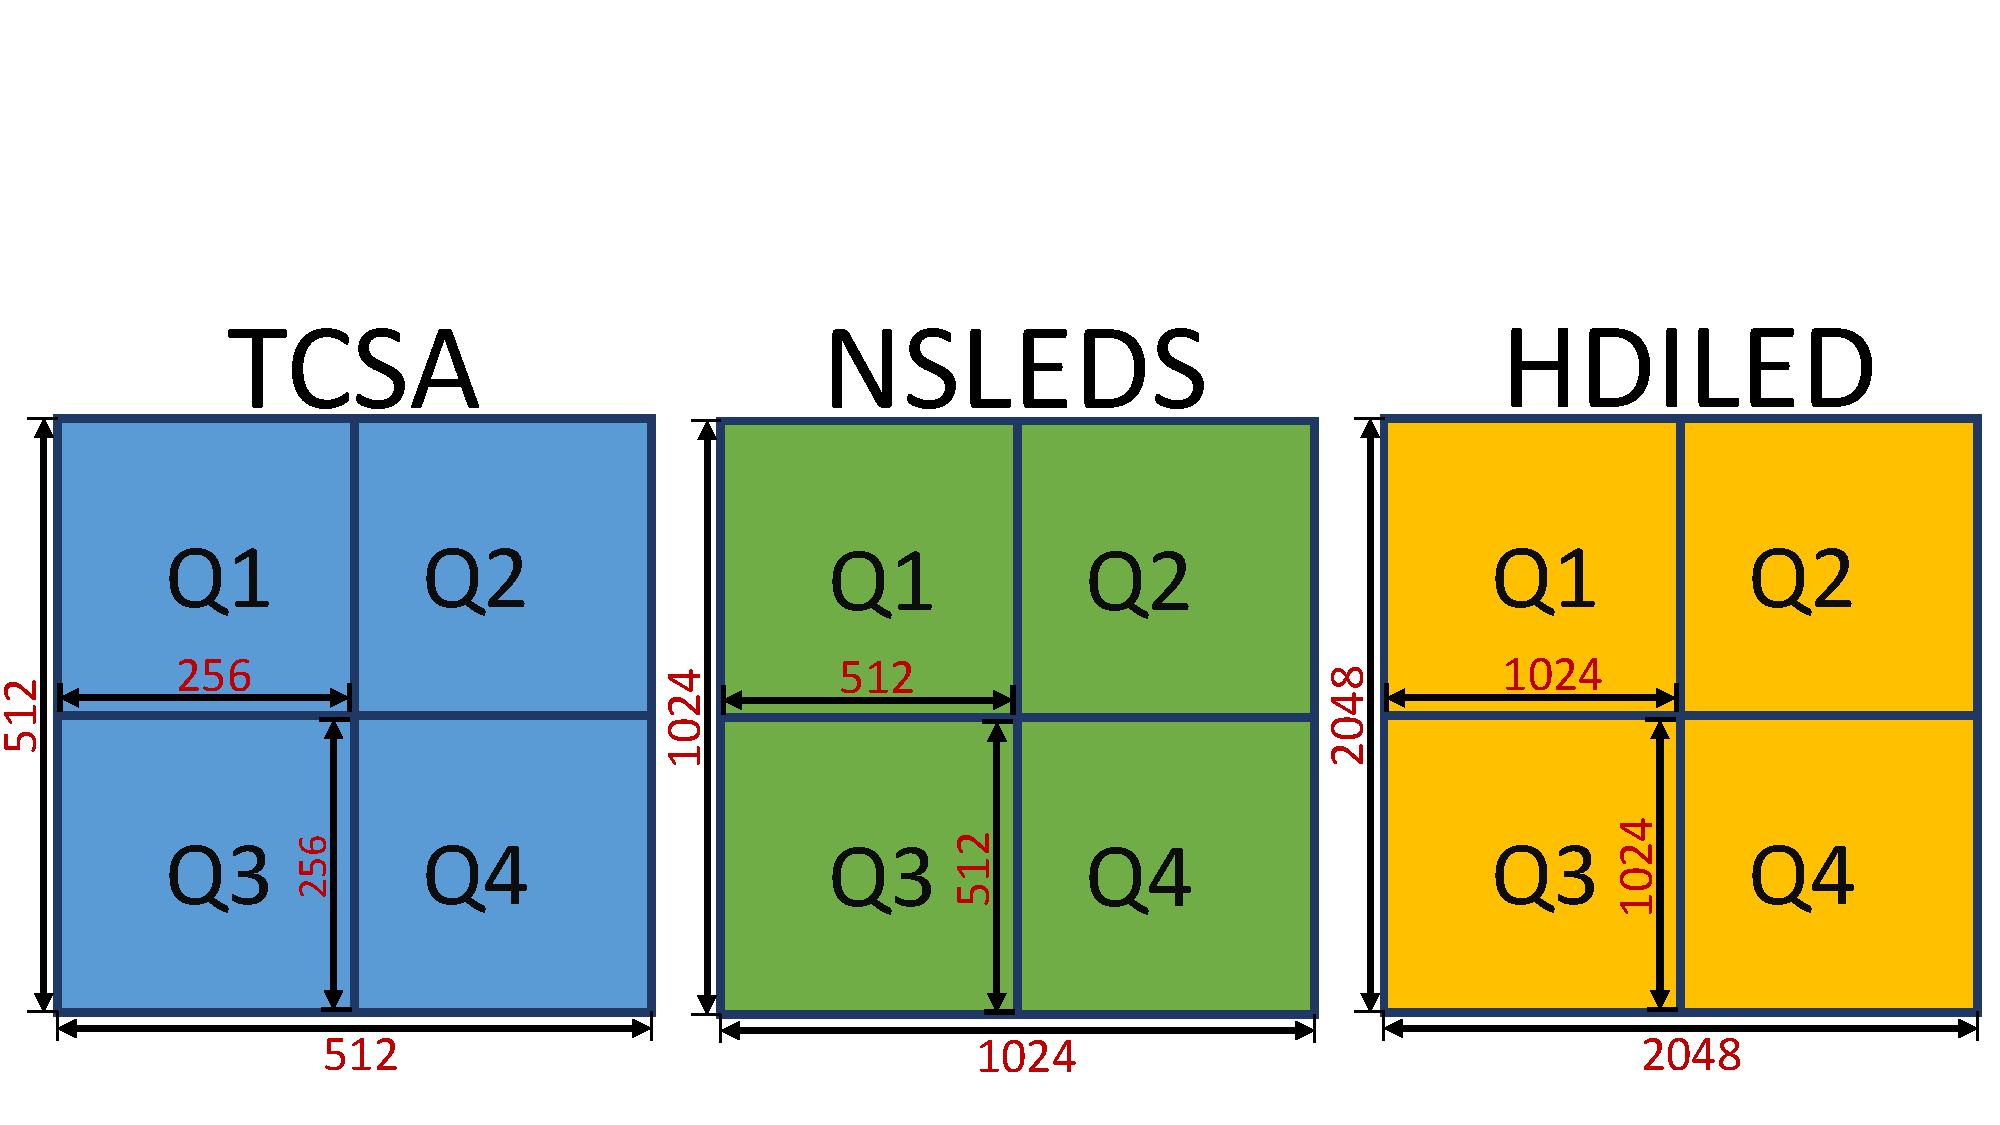
\includegraphics[trim=0in 0.35in 0in 1.5in,width=1.0\textwidth]{fig/tcsa_nsleds_hdiled_quads.pdf}
        \caption[TCSA, NSLEDS, and HIDLED Array Quadrant Layouts]{TCSA, NSLEDS, and HIDLED Array Quadrant Layouts\textsuperscript{a}}
        \vspace{-8px}
        \footnotesize\textsuperscript{a} Not drawn to scale
        \label{fig:tcsa_nsleds_hdiled_quads}
    \end{figure}

    The quadrant write enable selects which quadrant to drive. It is worth noting that each quadrant has separate internal signaling which allows for each quadrant to operate independently in parallel when mounted in a package that provides independent external signals. However, to date most of the fabricated IRLED arrays are mounted in packages that allows for only one quadrant to be drawn at a time\footnote{Currently, only HIDLED has been tested in the type of setup\cite{lassiter1, LassiterEtAl2019_1, LassiterEtAl2019_2, lassiter3} due to it having the largest resolution per quadrant.}. In a setup being driven in parallel, multiple CSEs are utilized. In a two CSE setup, half of the quadrant bits would be controlled by one CSE and half by another. In a four CSE setup, a single quadrant would be controlled by a single CSE. Irrespective of the number of CSEs used to a drive an array, the internal RIIC signal lines would be driven in precisely the same manner within each quadrant with the only change being that they operate asynchronously with respect to the others.

    The X address, Y address, and LOAD are used to select which pixel or group of pixels to write within a quadrant depending on the mode of operation. Though these lines are effectively shared by quadrants in a single CSE Setup, within the RIIC architecture they can be driven independently for each quadrant. Internally, each array can write up to 32 pixels (or channels) of data at a given time. The mode of operation dictates whether 2, 4, 8, 16, or 32 channels are used. The number of address bits utilized depends on the mode of operation. The amount of address bits differs by array due to the differences in sizes. NSLEDS utilizes 7 bits for the X address and 7 bits for the Y address, yielding a total of 256 by 256 addresses per quadrant. The LOAD bit is used to select between even and odd rows, yielding an effective address space of 256 by 512 per quadrant. Because the smallest mode of operation writes 2 pixels at a time, this is sufficient to fully address the array. Similarly, HDILED utilizes 8 bits for the X address and 8 bits for the Y address, yielding a total of 512 by 512 addresses per quadrant. Again, as with NSLEDS, the LOAD bit is used to select between even and odd rows, yielding an effective address space of 512 by 1024 per quadrant. This is again sufficient to completely address the array since it also can at a minimize write 2 pixels at a time.

    Structurally, NSLEDS and HIDLED are layed out as super pixel as shown in Figure~\ref{fig:nsleds_hdiled_array_superpixel_layout}. Each super pixel is made up of a grid of 4 pixels spanning two rows and columns. These are layed out across the array in a grid structure with NSLEDS consisting of 256 by 256 super pixels, and HIDLED consisting of 512 by 512 super pixels. This image also highlights two points discussed above, the LOAD line selects between the top two pixels (even rows) and bottom two pixels (odd rows) of each super pixel in the quadrant, and the two selected pixels are both written at the same time. Additionally, these share a drive strength as noted in the diagram. This is controlled using the Strong/Weak drive strength bits which dictate whether to provide a strong or weaker light emission for the given pair of pixels.

    \begin{figure}
        \centering
        %includegraphs[trim=L B R T]
        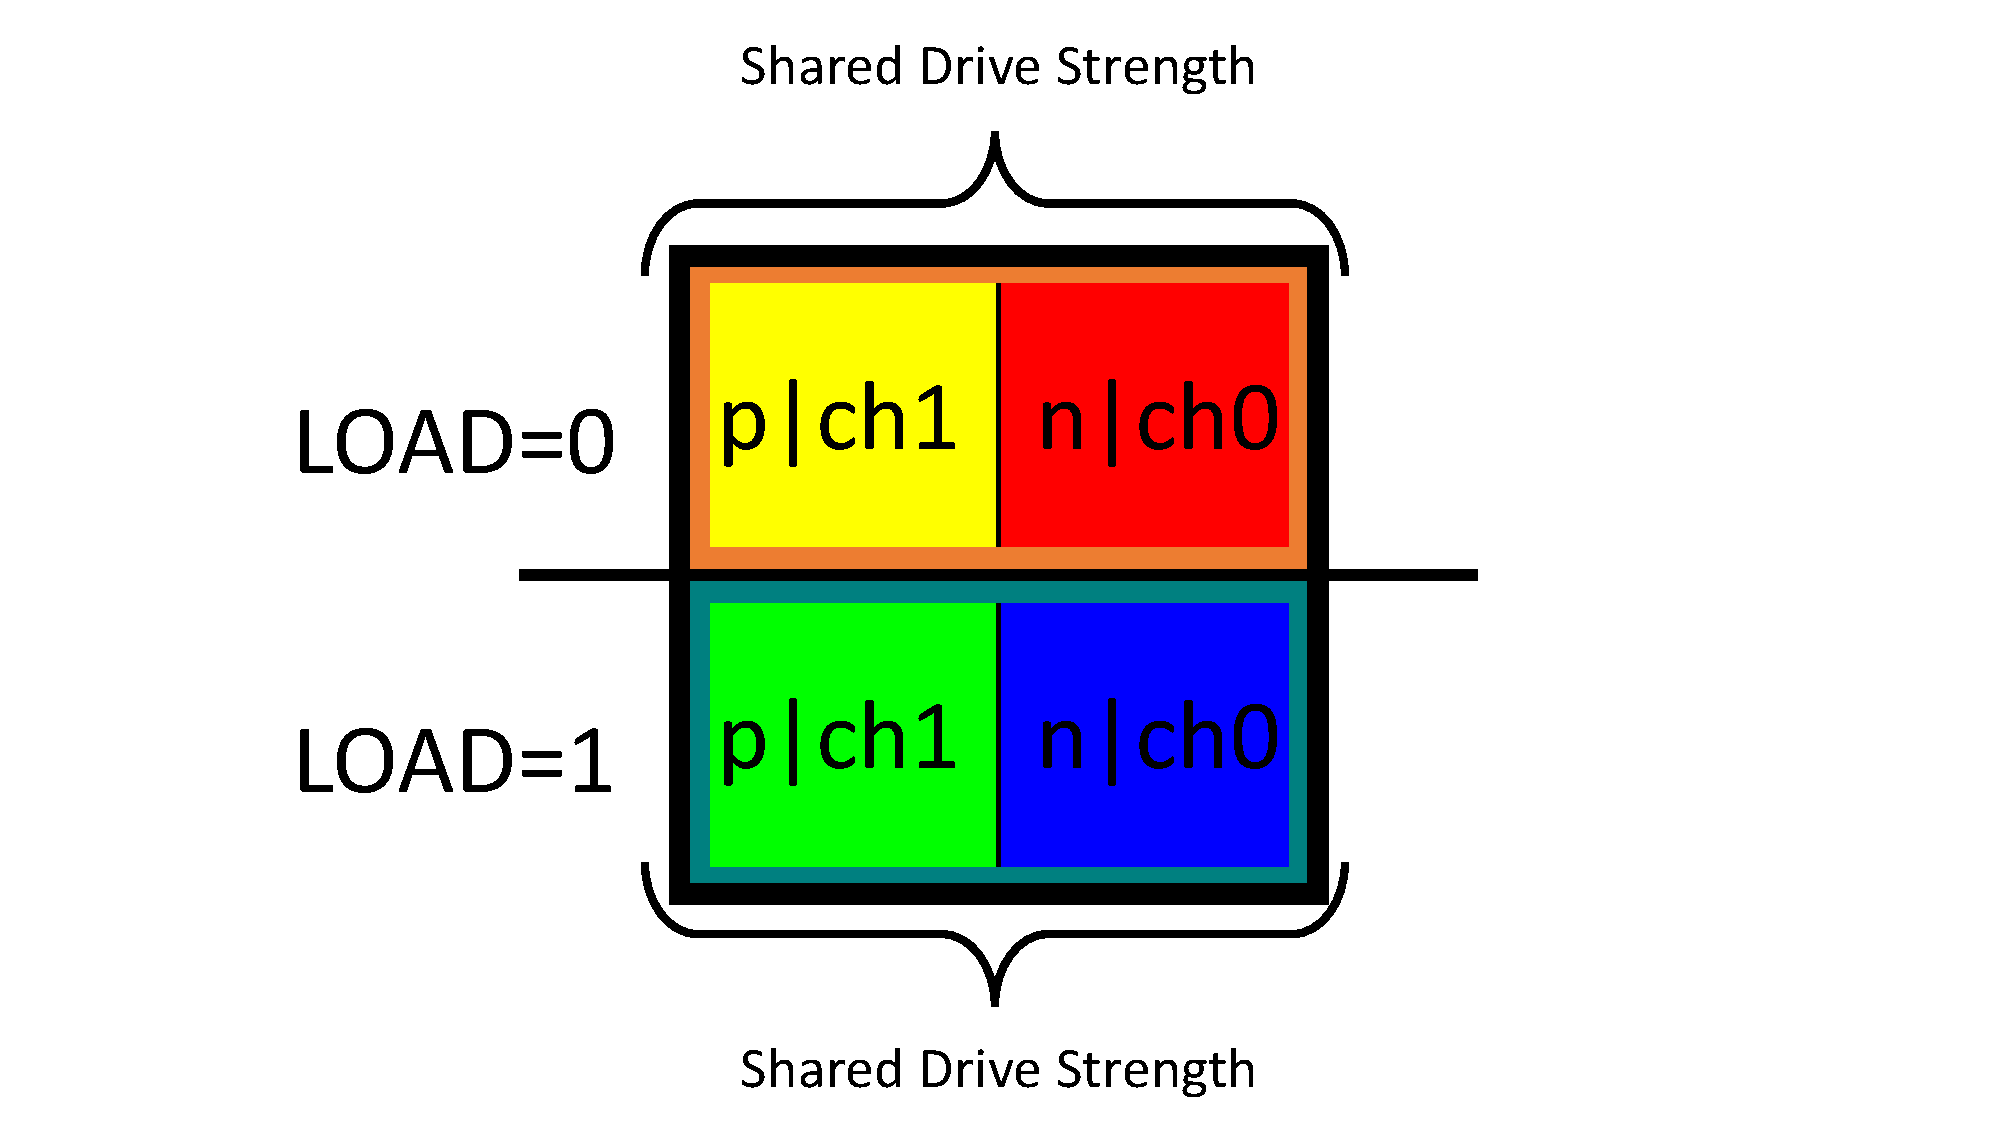
\includegraphics[trim=0in 0in 0in 0in,width=0.8\textwidth]{fig/superpixel_layout.pdf}
        \caption{NSLEDS/HDILED Array Super Pixel Layout}
        \label{fig:nsleds_hdiled_array_superpixel_layout}
    \end{figure}

    The 32 analog signaling lines control the emission intensity of driven pixels. These 32 channels are controlled by digital to analog converters within the CSE that are driven by the firmware. Internally, a CSE has 8 DAC cards with 2 DAC integrated circuits per card, with each DAC circuit consisting of 2 DAC channels as discussed in Section~\ref{sec:close_support_electronics}. Each channel is used to drive a single pixel, giving the ability to drive 32 pixels at once or some subset as mentioned previously.

    In practice, it is perferable to utilize all channels at once because this allows for more pixels to be driven in a shorter amount of time. Figure~\ref{fig:nsleds_hdiled_array_interleaved_pixel_mapping_per_write} shows the pixel mapping per write for 32 physical pixels on an array. 2 by 32 columns of pixels are shown segmented into super pixels. The Y address denotes the 16 super pixels that are selected per address. If Y is incremented by 1 then the next 16 rows of super pixels would be selected. X address (not shown) simply selects the next two columns of super pixels. DAC Card denotes which DAC card drives the given super pixel. L denotes which value of LOAD will select which columns within super pixels. When LOAD is low as shown in the middle segment, the top super pixels are selected as indicated in cyan. When LOAD is high as shown in the right segment, the bottom super pixels are selected.

    \begin{figure}
        \centering
        %includegraphs[trim=L B R T]
        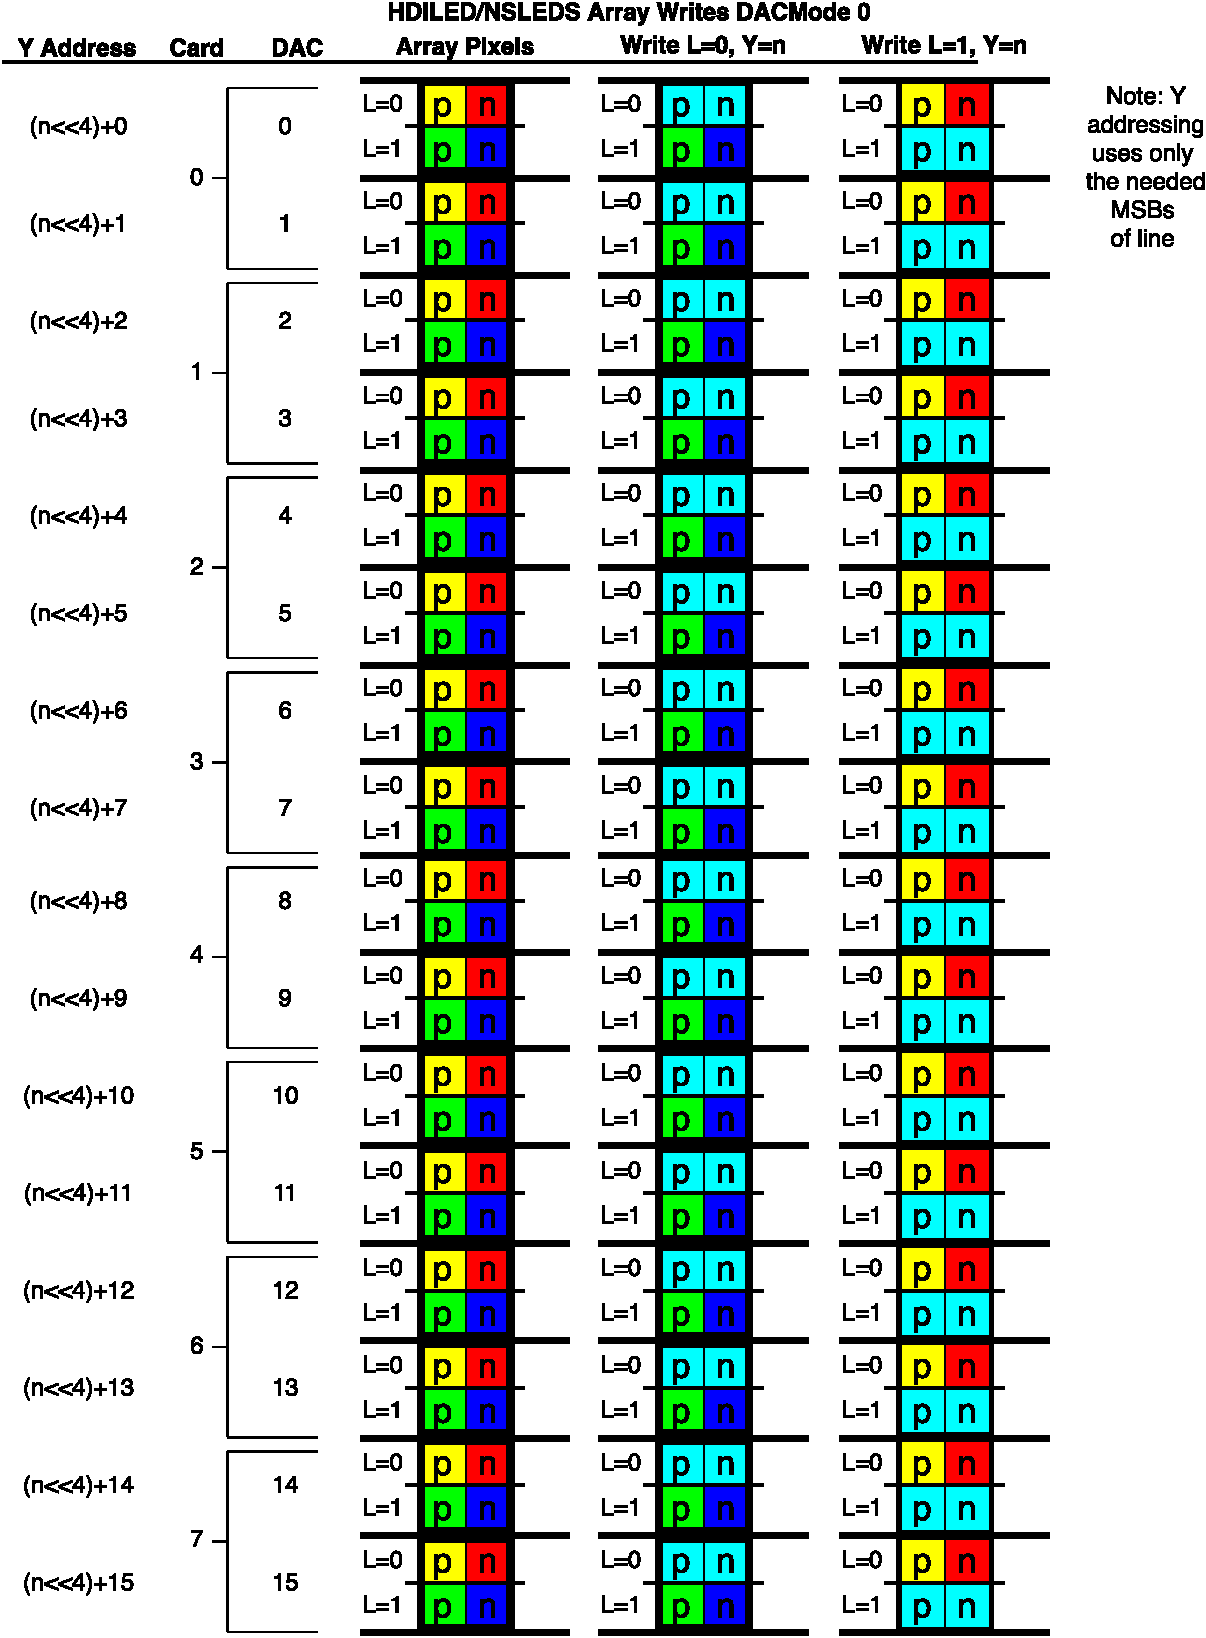
\includegraphics[trim=0in 0.3in 0in 0in,width=1.0\textwidth]{fig/nsleds_hdiled_array_writing.pdf}
        \caption{NSLEDS/HDILED Array Interleaved Pixel Mapping Per Write}
        \label{fig:nsleds_hdiled_array_interleaved_pixel_mapping_per_write}
    \end{figure}

    The overall writing process for writing 64 pixels is a two step process. First, 32 values for the even rows are loaded in and written to the array, followed by 32 values from the odd rows being loaded and written to the array. At a data level, it is ideal to interleave the data such that it is avaliable at the optimal time in order to reduce latency and buffering requirements within the firmware. This is discussed in detail in Chapter~\ref{chap:pdp_protocol}.

    Writing additional segments of pixels largely means buffering more data and repeating the same write process while asserting the correct address lines. Given that the arrays have no inherit hardware required write order other than what has been discussed above, the exact order of writing independent segments of 32 pixels can change depending on a number of factors. In a single CSE Setup, under most circumstances, the data for the top quadrants is carried by a single HDMI input going into a CSE, and the data for the bottom quadrants carried by the other HDMI input\footnote{When utilizing PDP for driving an array the location of where data is to be written on an array is agnostic to the HDMI input the data is carried on.}. In this case, the CSE firmware will swap between writing segments of 32 or 64 pixels to the top and bottom halves of an array. The former if it is desirable to write a minimal amount of data before servicing data from another input, the latter if it is desirable to complete an entire chunk of pixels. In a two CSE Setup, data over the hdmi links data could be segmented either horizontally or vertically meaning that each HDMI link would carry an entire quadrants data. In a four CSE setup, each link would carry half a quadrants data. As the reader may imagine, the order of writes could be configured in many different ways under these scenerios. Though it will not be discussed in detail within this thesis, it is worth noting for posterity that the order of writes on IRLED arrays does affect the thermal load on an array which has an effect on pixel brightness; thus, controlling the order of writes can be an important factor to consider for designers and users of a system.

\section{Classical Display Protocols}
    \label{sec:classical_display_protocols}

    Classical display protocols such as (DVI\cite{DDWG1999}, HDMI\cite{HDMIForum2018}, and DisplayPort\cite{VESA2016} are commonly used for driving consumer electronic devices. These generally provide a standardized feature-set that is rooted in classical analog video specifications (e.g. VGA, Composite)\cite{NIAnalog} that utilize scan lines\cite{Neal1998}. Scan lines are used to provide video timing information in order to synchronize a display to a given refresh-rate. Each scan line consist of an active video region followed by a horizontal blanking period. After all active video scan lines are displayed, a vertical synchronization region is used to indicate the end of a frame.

    \begin{figure}
        \centering
        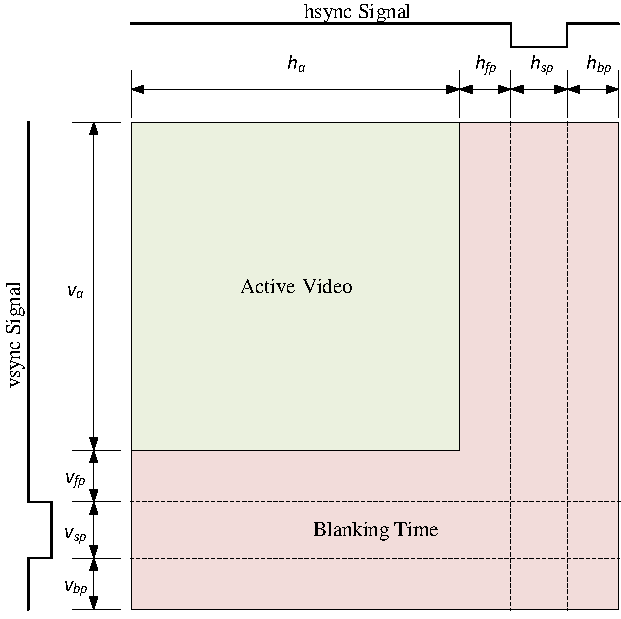
\includegraphics[width=0.9\textwidth]{fig/display_timing_overview.pdf}
        \caption{Display Protocol Timing Overview}
        \label{fig:display_protocol_timing_overview}
    \end{figure}

    \begin{figure}
        \centering
        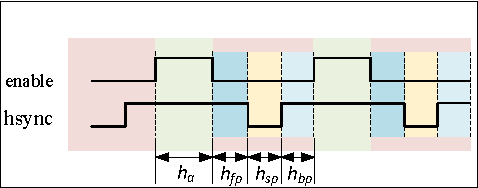
\includegraphics[width=0.7\textwidth]{fig/display_timing_line_cross.pdf}
        \caption{Display Protocol Horizontal Signal Cross Section Timing}
        \label{fig:display_protocol_line_cross}
    \end{figure}

    %FIXME add crosssectional blowout chart

    An overview of this is shown in Figure~\ref{fig:display_protocol_timing_overview}. The region shown in green is the pixel data for the active video region of the display. It is of size $H_a\times V_a$ which represents the number of pixels to display, for example, 1920 by 1080 for a HDTV high-definition video mode\cite{MythTVWebsite}. The blanking time regions denote pixel data that is sent but not displayed\footnote{Typically data lines are held low during this period, but somtimes it is used for out-of-band communication to send other information such as audio encoding.}. A scan line consist of pixels made up of $h_a$, the horizontal active size; $h_{fp}$, the horizontal front porch before the pulse signal; $h_{sp}$, the horizontal sync pulse; and $h_{bp}$, the horizontal back porch after the sync pulse. The vertical blanking period makes up multiple scanlines and consist of $v_{fp}$, the vertical front porch before the vsync pulse; $v_{sp}$, the vertical sync pulse; $v_{bp}$, the vertical back porch after the vertical sync pulse. Sync pulses are generally active low, meaning that during active display a sync signal is high as shown in the diagram.

    Figure~\ref{fig:display_protocol_line_cross} shows a closeup view of signal lines during the active region of display for two scan lines. A data enable signal denoted by $enable$ is high during the active region shown in green. Following this, it goes low for a period of time denoted by $h_{fp}+h_{sp}+h_{bp}$. The horizontal sync signal goes low only in the region shown in yellow between the front porch and back porches. This process repeats for all scan lines. Once the last active region pixel is drawn, the enable signal will stop going high during the vertical synchronization period.

    %FIXME: Fix discussion of DP not using fucking backwards compatibility shitty hdmi fucking mode
    %FIXME: Talk about CC in the vertical blanking

    \begin{figure}
        \centering
        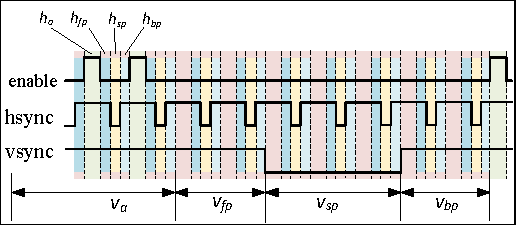
\includegraphics[width=0.9\textwidth]{fig/display_timing_full_cross.pdf}
        \caption{Display Protocol Full Signal Cross Section Timing}
        \label{fig:display_protocol_full_cross}
    \end{figure}

    Figure~\ref{fig:display_protocol_full_cross} shows a closeup view of signal lines during the transition into the vertical synchronization period. The region donated by $V_a$ indicates the end of the video active region of the display which occurs toward the end of a frame. After the active video region, all data has been drawn to a display. The region denoted by $v_{fp}+v_{sp}+v_{bp}$ is the vertical blanking or vsync period during which no active video data is sent; therefore, data enable denoted by $enable$ is always low during this period. Before the vertical sync pulse period denoted by $v_{sp}$ occurs, a vertical front porch period denoted by $v_{fp}$ occurs. After the vertical sync pulse, a vertical back porch region $v_{bp}$ occurs. Following this the beginning of the next frame occurs as denoted by $v_{a+1}$.
    \begin{figure}
        \centering
        { \Large
            $l_h=h_a+h_{fp}+h_{sp}+h_{bp}$ \vspace{8px} \\
            $l_v=v_a+v_{fp}+v_{sp}+v_{bp}$ \vspace{8px} \\
            $f_f={f_p \over {l_h \cdot l_v}}$ \\
            $p_t={1 \over f_p}$ \vspace{8px} \\
            $f_t={1 \over f_f}$ \vspace{8px}
        }
        \caption{Total Refresh Rate}
        \label{fig:modeline_refresh_rate}
    \end{figure}

    Figure~\ref{fig:modeline_refresh_rate} shows the relationship between between the different regions of a display and the frequency or refresh rate. $l_h$ denotes the scan line size of a display, or total horizontal width, which is made up of the horizontal active and horizontal porch region pixels of a display. $l_v$ denotes the total vertical width of a display, which is made up the vertical active and vertical porch region pixels of a display. Each pixel is sent at a rate denoted by $f_p$, the pixel frequency (also called the pixel clock). $f_f$ denotes the frame frequency or framerate of a display. This is simply the pixel frequency over the total number of pixels (video active and porches) of a display. $p_t$ denotes the time period a single pixel takes to send. $f_t$ denotes the time period for an entire frame.

    %FIXME: example modeline
    To illustrate, let us look at the display modeline generated using the VESA Coordinated Video Timing (CVT) standard shown in Figure~\ref{fig:modeline_example}. This modeline operates a total frame frequency of approximately \mbox{30 Hz}. The pixel clock 79.75, denoted in red, is specified in megahertz. The horizontal pixels, denoted in blue; are the end of horizontal active, the end of horizontal front porch, the end of horizontal sync pulse, and the end of horizontal back porch respectively. The vertical pixels (measured in lines), denoted in green; are the end of vertical active, the end of vertical front porch, the end of vertical sync pulse, and the end of horizontal back porch respectively. The sync pulse polarities, denoted in yellow; indicate whether a given sync pulse is active low or active high. A minus symbol indicates active low and a plus symbol indicates active high. If these numbers are placed into into the formulas shown in Figure~\ref{fig:modeline_refresh_rate} the results shown in Figure~\ref{fig:modeline_refresh_rate_plug} are yielded. The astute reader will note that $l_h$ and $l_v$ are the same as the total pixel size for the given modeline. The pixel period is $\sim12.53 ns$, meaning that each pixel is drawn for the given amount of time. The frame period is $\sim33.33 ms$, meaning that each frame is drawn for that given amount of time.

    \begin{figure}
        \centering
        { \normalsize
        \textbf{``1920x1080\_30.00"} {\color{red}79.75}  {\color{blue} 1920 1976 2168 2416}  {\color{darkgreen}1080 1083 1088 1102} {\color{olive}-hsync +vsync}
        %\vspace{-8px}
        }
        \caption{VESA CVT Generated Modeline}
        \label{fig:modeline_example}
    \end{figure}

    %FIXME: finish this chart
    \begin{figure}
        \centering
        { \Large
            $h_a=1920; h_{fp}=1976-h_a; h_{sp}=2168-h_{fp}; h_{bp}=2416-h_{sp};$ \\
            $v_a=1080; v_{fp}=1083-v_a; v_{sp}=1088-v_{fp}; v_{bp}=1102-v_{sp};$ \\
            $l_h=2416=1920+56+192+248$ \vspace{8px} \\
            $l_v=1102=1080+3+5+14$ \vspace{8px} \\
            $f_p=79.75e6$ \vspace{8px} \\
            $f_f=30.0={f_p \over {l_s \cdot l_c}}$ \\
            $p_t=12.53ns={1 \over f_p}$ \vspace{8px} \\
            $f_t=33.33ms={1 \over f_f}$ \vspace{8px}
        }
        \caption{Computed Refresh Rate for a 30Hz CVT Modeline}
        \label{fig:modeline_refresh_rate_plug}
    \end{figure}

    Section~\ref{sec:displays_within_proj_system}, discusses how these protocols are utilized within an IRLED projector system, briefly highlight the limitations, and . %FIXME: finish this paragraph

\section{Display Protocols within an IRLED Project System}
    \label{sec:displays_within_proj_system}
    Projector systems utilize
